\documentclass[12pt]{article}
\usepackage{setspace,graphicx,amsmath,geometry,fontspec,titlesec,soul,bm,subfigure}
\titleformat{\section}[block]{\LARGE\bfseries}{\arabic{section}}{1em}{}[]
\titleformat{\subsection}[block]{\Large\bfseries\mdseries}{\arabic{section}.\arabic{subsection}}{1em}{}[]
\titleformat{\subsubsection}[block]{\normalsize\bfseries}{\arabic{subsection}-\alph{subsubsection}}{1em}{}[]
\titleformat{\paragraph}[block]{\small\bfseries}{[\arabic{paragraph}]}{1em}{}[]
\setmainfont{Times New Roman}
\renewcommand{\baselinestretch}{1.15}
\geometry{a4paper,left=2.5cm,right=2.5cm,top=2.5cm,bottom=2.5cm}
\begin{document}
	\newpagestyle{main}{            
		\sethead{Ziqing Yu}{Bildverarbeitung 2}{3218051}     
		\setfoot{}{\thepage}{}
		\headrule
		\footrule
			}
	\pagestyle{main}

Der RGB-Bild und der panchromatische Bild
\begin{figure}[ht]\centering
	\subfigure[panchromatischerBild]{
		\includegraphics[width=0.45\textwidth]{DMC_haeuser_pan.bmp}}
	\subfigure[RGB-Bild]{
		\includegraphics[width=0.45\textwidth]{DMC_haeuser_lowRGB_original.bmp}}
\end{figure}
\newline
Bilder im RGB Frabraum werden in 3 Matrizen Repräsentiert wo die Grauwerten für Rot, Grün und Blau gespeichert werden. Farbraum HSV ist ein intuitive Repräsentation, wobei H für Hue, S für Saturation und V für Value(Intensität auf Deutsch) stehen. Hue beschreibt die Qualität der Farbe, Saturation beschreibt die Reinheit der Farbe und die Intensität beschreibt die Helligkeit der Farbe. Die Formel der Transformation zwischen dieser 2 Farbräume lautet, \newline
\newline
Transformation RGB in HSV. Zunächst werden Grauwerten nominiert. 
\begin{equation*}
H = \begin{cases} \Theta \\ 2 \pi - \Theta,\end{cases}
\end{equation*}
\begin{equation*}
mit\ \  \ \  \Theta = \arccos  \frac {\frac{1}{2} \cdot [(R-G)+(R-B)]} {[(R-G)^2+(R-G)(G-B)]^{\frac{1}{2}}} 
\end{equation*}
\begin{equation*}
S = 1- \frac{3}{(R + G + B)} [min (R, G, B)]
\end{equation*}
\begin{equation*}
I = \frac{1}{3} (R + G + B)
\end{equation*}
\clearpage
\begin{figure}\centering
\begin{tabular}[ht]{lll}
\hline
\multicolumn{1}{|l|}{Für$\ 0° < H \leq 120°]$} & \multicolumn{1}{l|}{Für$\ 120° < H \leq 240°]$}    & \multicolumn{1}{l|}{Für$\ 240° < H \leq 360°]$}         \\ \hline
\multicolumn{1}{|l|}{}          & \multicolumn{1}{l|}{$H = H - 120°$} & \multicolumn{1}{l|}{$H = H - 240°$} \\ \hline
\multicolumn{1}{|l|}{$B = I (1 - S)$}          & \multicolumn{1}{l|}{$R = I (1 - S)$} & \multicolumn{1}{l|}{$G = I (1 - S)$} \\ \hline
\multicolumn{1}{|l|}{$R = I [1 + \frac{S(\cos H)}{\cos(60° - H)}]$}          & \multicolumn{1}{l|}{$G = I [1 + \frac{S(\cos H)}{\cos(60° - H)}]$} & \multicolumn{1}{l|}{$B = I [1 + \frac{S(\cos H)}{\cos(60° - H)}]$} \\ \hline
\multicolumn{1}{|l|}{$G = 3I - (R + B)$}          & \multicolumn{1}{l|}{$3I - (R + G)$} & \multicolumn{1}{l|}{$3I - (G + B)$} \\ \hline
\end{tabular}
\caption{Transformation HSV in RGB }
\end{figure}
Zuerst wird der alte RGB Bild in HSV Farbraum transformiert, dann ersetzt man die Intensität durch panchromatisches Bild höher Auflösung, danach wird Bild in HSV Farbraum in RGB Raum rücktransformiert und man bekommt 3 RGB Kanäle, am Ende werden neue RGB Kanäle zusammenbindet und der Bild mit höher Auflösung ist erzeugt. 
\begin{figure}[ht]\centering
	\subfigure[Kanal Rot]{
		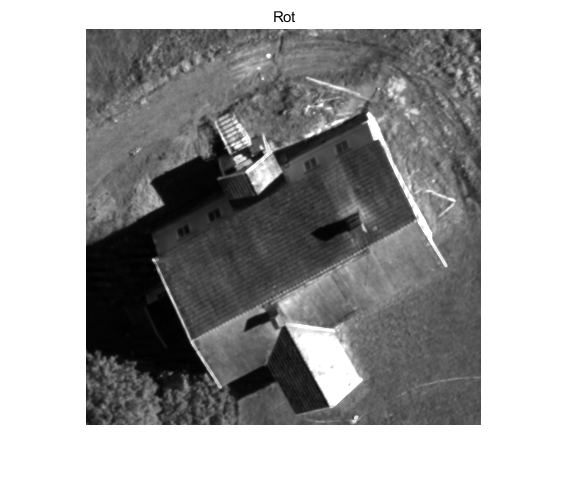
\includegraphics[width=0.45\textwidth]{Rot.png}}
	\subfigure[Knal Grün]{
		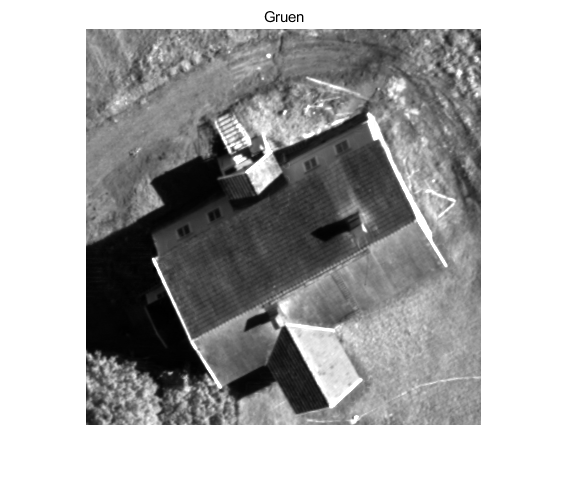
\includegraphics[width=0.45\textwidth]{Gruen.png}}
	\subfigure[Knal Blau]{
		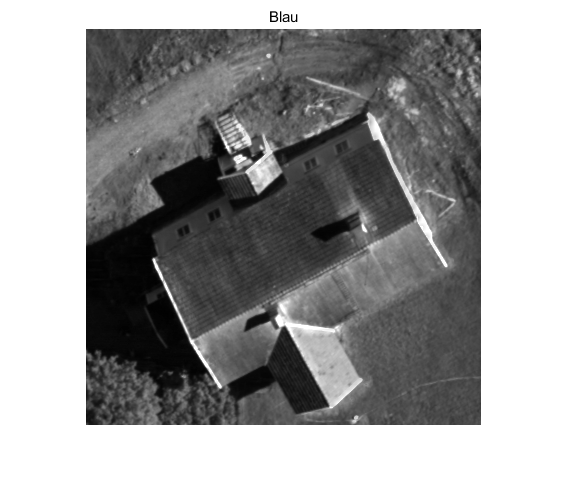
\includegraphics[width=0.45\textwidth]{Blau.png}}
	\subfigure[neuer RGB-Bild]{
		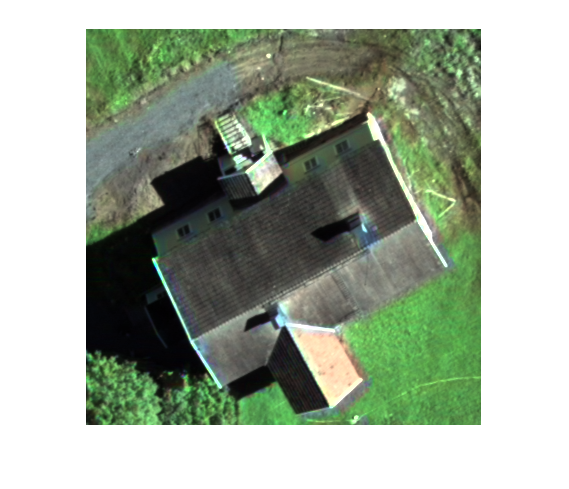
\includegraphics[width=0.45\textwidth]{FinalBild.png}}
\end{figure}

\end{document}